\documentclass[12pt, a4paper, oneside]{ctexart}
\usepackage{amsmath, amsthm, amssymb, bm, color, framed, graphicx, hyperref, mathrsfs, float, caption,subfigure}
\usepackage[justification=centering]{caption}

% multi-column
\usepackage{tasks}
% itemize
\NewTasksEnvironment[label=(\arabic*), label-width=3ex]{exercise}
%\settasks{
% label = \theexercise.\arabic* ,
% item-indent = 2em ,
% label-width = 2em ,
% label-offset = 0pt
%}

\everymath{\displaystyle}

\title{\textbf{第七次作业}}
\author{U08M11002 Fall 2023}
\linespread{1}
\definecolor{shadecolor}{RGB}{241, 241, 255}

\newcounter{problemname}
\newenvironment{problem}{\stepcounter{problemname}\par\noindent\textbf{题目\arabic{problemname}. }}{\\\par}
\newenvironment{warning}{\begin{shaded}\par\noindent\textbf{提交作业方式:}}{\end{shaded}\par}

\begin{document}
	
\maketitle
	
\hspace{1em}

\begin{problem}
	已知系统相应的齐次方程及其对应的 $0_+$ 时刻的状态条件,求系统的零输入响应。
	\begin{exercise}(1)
		\task $\frac{d^2}{d^2t} y(t) + 2 \frac{d}{dt} y(t) + 2y(t) = 0$,$r(0_+)=1,r'(0_+)=2$
		\task $\frac{d^2}{d^2t} y(t) + 2 \frac{d}{dt} y(t) + y(t) = 0$,$r(0_+)=1,r'(0_+)=2$
		\task $\frac{d^3}{d^3t} y(t) + 2\frac{d^2}{d^2t} y(t) +  \frac{d}{dt} y(t) + 2y(t) = 0 $,$r(0_+)=r'(0_+)=0,r''(0_+)=1 $
	\end{exercise}
	\quad
\end{problem}

	
\begin{problem}
	如下图所示的 RC 电路中,已知 $R = 1 \Omega, C=0.5F$,写出描述该系统的微分方程。电容的初始状态 $u_{C}(0_-) = u_{C}(0_+) = -1V$, 求激励 $u_s(t)$ 为下列信号时的电容 $C$ 的电压全响应 $u_C(t)$:
	\begin{figure}[H]
		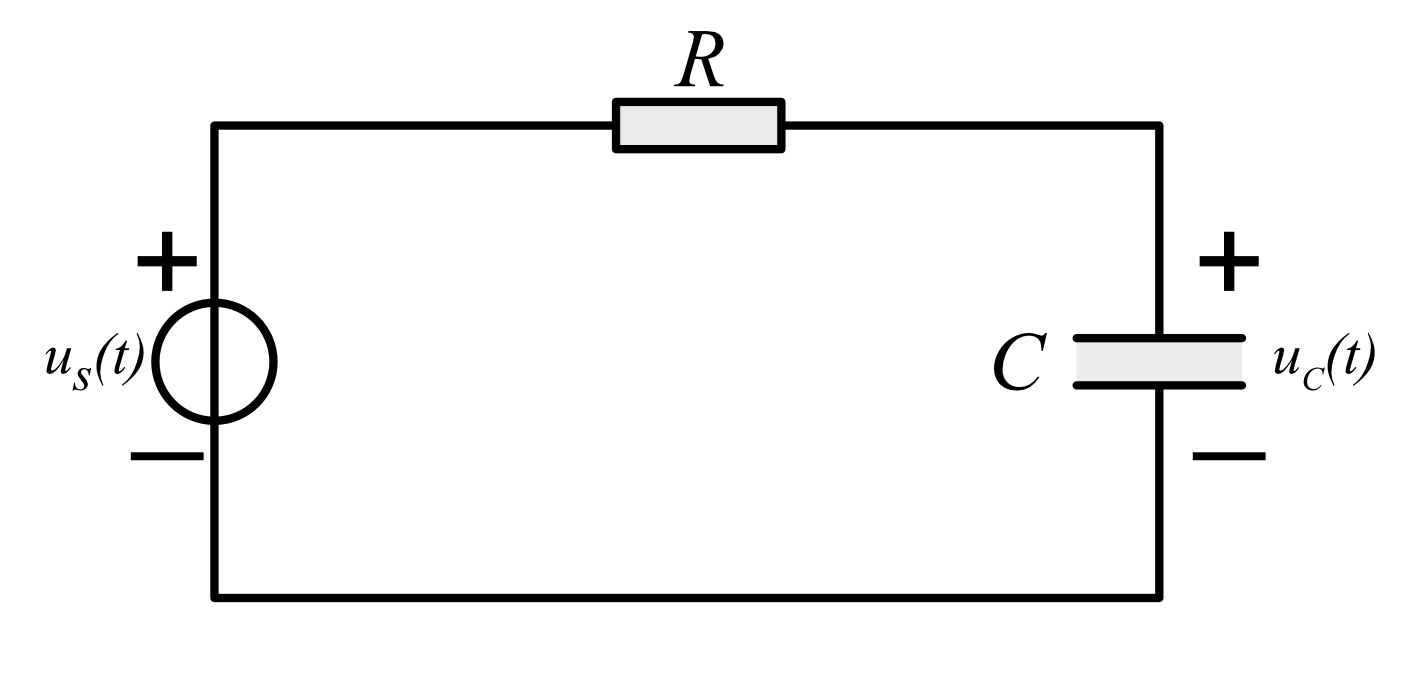
\includegraphics[width=8cm]{assets/hw2img1.png}
		\centering
	\end{figure}
	\begin{exercise}(2)
		\task $u_s(t) = U(t)$
		\task $u_s(t) = e^{-t}U(t)$
		\task $u_s(t) = e^{-2t}U(t)$
		\task $u_s(t) = tU(t)$
	\end{exercise}
	\quad
\end{problem}

\begin{problem}
	描述某 LTI 系统的微分方程为 $y''(t) + 3 y'(t) + 2y(t) = 2f'(t) + 6 f(t)$,已知$y(0^-)=2$,$y'(0^-)=0$,$f(t)=U(t)$,求 $y(0^+)$ 和 $y'(0^+)$。
	\quad
\end{problem}
	
	
\begin{problem}
	对上题所描述的系统和起始条件,求该系统的零输入响应、零状态响应和全响应。
	\quad
\end{problem}
	
\begin{problem}
	上题所描述的系统,如果不知道起始条件,只知道初始条件$y(0^+)=3$,$y'(0^+)=1$,$f(t)=U(t)$,求该系统的零输入响应、零状态响应。
	\quad
\end{problem}
	

\begin{problem}
	描述某 LTI 系统的微分方程为 $y'(t) + 2 y(t) = f''(t) + f'(t) + 2f(t)$,若$f(t)=U(t)$,求该系统的零状态响应。
	\quad
\end{problem}
	
	
\begin{problem}
	已知某 LTI 系统的常微分方程为 $y'(t) + y(t) = f(t)$,
	\begin{exercise}(1)
		\task 若完全响应为$y(t)=[5e^{-t} + 3e^{-2t}]U(t)$,且$y(0^-)=5$,求该系统的零输入响应和零状态响应;
		\task 若$y(0^-)=10$,求系统的零输入响应;
		\task 若完全响应为$y(t)=[5e^{-t} + 3e^{-2t}]U(t)$,且$y(0^-)=5$,求$y'(t) + y(t) = f(t-2)$的零状态响应;
		\task 若完全响应为$y(t)=[5e^{-t} + 3e^{-2t}]U(t)$,且$y(0^-)=5$,求$y'(t) + y(t) = f'(t) + 2f(t)$的零状态响应。
	\end{exercise}
	\quad
\end{problem}
	
\begin{problem}
	已知描述系统的微分方程和起始状态如下,求零输入响应、零状态响应和全响应(从特征根求响应可以查表)。
	\begin{exercise}(1)
		\task $y''(t) + 4 y'(t) + 3y(t) =  f(t)$, $y(0^-)=1$,$y'(0^-)=1$,$f(t)=U(t)$
		\task $y''(t) + 4 y'(t) + 4y(t) =  f'(t) + 3 f(t)$, $y(0^-)=1$,$y'(0^-)=2$,$f(t)=e^{-t}U(t)$
		\task $y''(t) + 2 y'(t) + 2y(t) =  f'(t) $, $y(0^-)=0$,$y'(0^-)=1$,$f(t)=U(t)$
	\end{exercise}
	\quad
\end{problem}
	
\begin{problem}
	求上题中各系统的冲激响应。
	\quad
\end{problem}

\newpage

\begin{problem}
	如下图所示电路,已知 $R=3\Omega$, $L=1H$, $C=0.5F$, $u_S(t)=\cos t U(t)V$, 求 $u_C(t)$ 的零状态响应。
	\begin{figure}[H]
		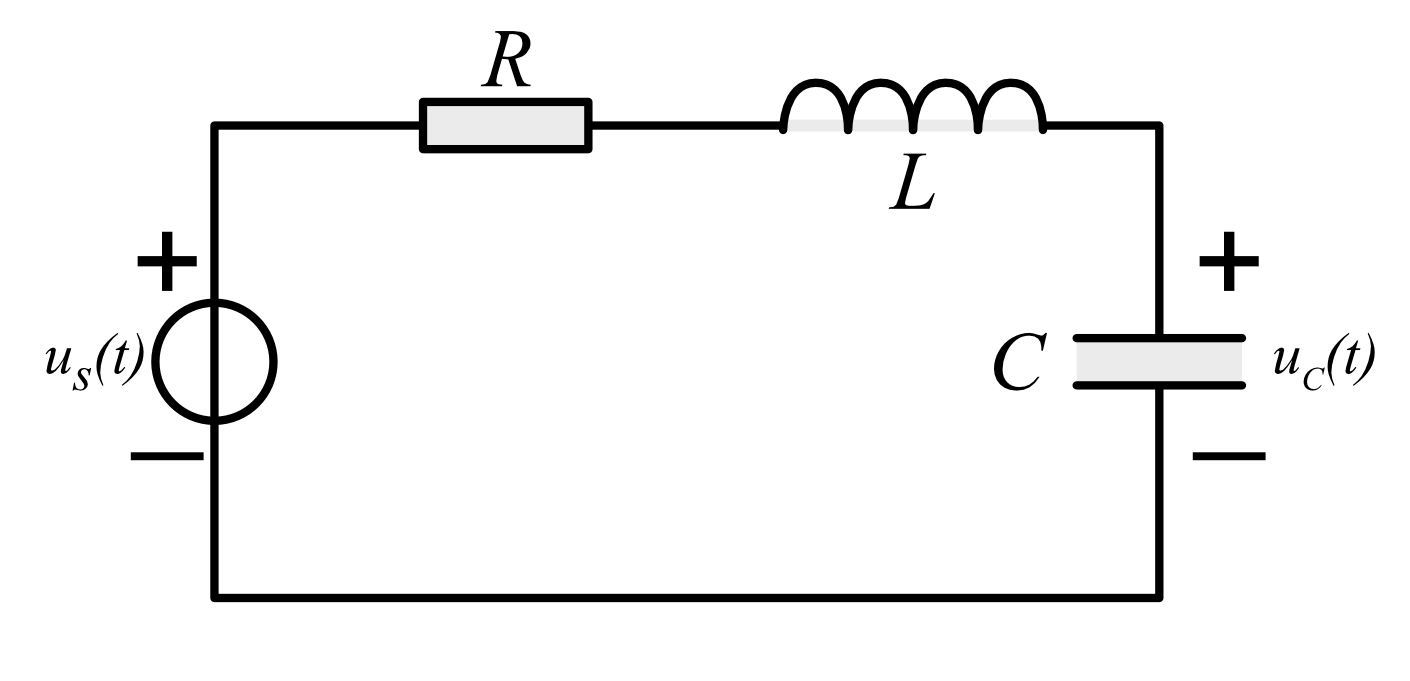
\includegraphics[width=8cm]{assets/hw3img2.png}
		\centering
	\end{figure}
	\quad
\end{problem}
	
	
\begin{problem}
	描述某二阶 LTI 系统的微分方程为 $y''(t) + 5y'(t) + 6y(t) = f(t)$,求冲激响应 $h(t)$。
	\quad
\end{problem}
	
	
\end{document}